% *****************************************************************************************************
% ****************************              SIMPLE EXAMPLE             ********************************
% *****************************************************************************************************

% =======================================================
% =======         HEADER FOR DOCUMENT        ============
% =======================================================
    
    % *********  SPECIFIC FOR THIS BOOK  ********
    \def\ProjectAuthorLink{https://github.com/CompilandoConocimiento}
    \def\ProjectNameLink{\ProjectAuthorLink/LibroProbabilidad}    
    

    % *********   DOCUMENT ITSELF   **************
    \documentclass[fleqn, journal, onecolumn]{IEEEtran}             %Type of doc and size of font and left equations
    \usepackage{ifthen}                                             %Allow simple programming using if - then
    \usepackage[hidelinks]{hyperref}                                %Allow to create hiperlinks and Fuck Firefox
    \usepackage{pdfpages}                                           %Allow us 'import' PDF's
    \hypersetup{pageanchor=false}                                   %Solve 'double page 1' warnings in build :v
    \setlength{\parindent}{0pt}                                     %Eliminate ugly indentation
    \author{Oscar Andrés Rosas}                                     %Who I am

    % *********   LANGUAJE    *****************
    \usepackage[english]{babel}                                     %Please allow me to type in spanish
    \usepackage[utf8]{inputenc}                                     %Lets use UFT-8
    \usepackage[T1]{fontenc}                                        %Allow for better font support
    \usepackage{textcmds}                                           %Allow us to use quoutes
    \usepackage{changepage}                                         %Allow us to use identate paragraphs
    \usepackage{anyfontsize}                                        %All the sizes for fonts wiiiii!

    % *********   MATH AND HIS STYLE  *********
    \usepackage{ntheorem, amsmath, amssymb, amsfonts}               %All fucking math, I want all!
    \usepackage{mathrsfs, mathtools, empheq}                        %All fucking math, I want all!
    \usepackage{cancel}                                             %Negate symbol
    \usepackage{centernot}                                          %Allow me to negate a symbol

    % *********   GRAPHICS AND IMAGES *********
    \usepackage{graphicx}                                           %Allow to create graphics
    \usepackage{float}                                              %For images
    \usepackage{wrapfig}                                            %Allow to create images
    \graphicspath{ {Graphics/} }                                    %Where are the images :D

    % *********   LISTS AND TABLES ***********
    \usepackage{listings, listingsutf8}                             %We will be using code here
    \usepackage[inline]{enumitem}                                   %We will need to enumarate
    \usepackage{tasks}                                              %Horizontal lists
    \usepackage{longtable}                                          %Lets make tables awesome
    \usepackage{booktabs}                                           %Lets make tables awesome
    \usepackage{tabularx}                                           %Lets make tables awesome
    \usepackage{multirow}                                           %Lets make tables awesome
    \usepackage{multicol}                                           %Create multicolumns

    % *********   REMOVE SOME ERRORS **********
    \hbadness=10000                                                 %Ignore \vbox and \hbox warings
    \hfuzz=\maxdimen\newdimen\hfuzz                                 %Ignore \vbox and \hbox warings

    
% =======================================================
% ===================   COMMANDS    =====================
% =======================================================

    % =========================================
    % =======   NEW ENVIRONMENTS   ============
    % =========================================
    \newenvironment{Indentation}[1][0.75em]                         %Use: \begin{Inde...}[Num]...\end{Inde...}
        {\begin{adjustwidth}{#1}{}}                                 %If you dont put nothing i will use 0.75 em
        {\end{adjustwidth}}                                         %This indentate a paragraph
    
    \newenvironment{SmallIndentation}[1][0.75em]                    %Use: The same that we upper one, just 
        {\begin{adjustwidth}{#1}{}\begin{footnotesize}}             %footnotesize size of letter by default
        {\end{footnotesize}\end{adjustwidth}}                       %that's it
    
    \def \Eq {equation}                                             %Stupid Visual studio error
    \newenvironment{MultiLineEquation}[1]                           %Use: To create MultiLine equations
        {\begin{\Eq}\begin{alignedat}{#1}}                          %Use: \begin{Multi..}{Num. de Columnas}
        {\end{alignedat}\end{\Eq}}                                  %And.. that's it!
    
    \newenvironment{MultiLineEquation*}[1]                          %Use: To create MultiLine equations
        {\begin{\Eq*}\begin{alignedat}{#1}}                         %Use: \begin{Multi..}{Num. de Columnas}
        {\end{alignedat}\end{\Eq*}}                                 %And.. that's it!

    \newenvironment{largeEq} {\begingroup \large}{\endgroup}        %Make eq bigger
    \newenvironment{LargeEq} {\begingroup \Large}{\endgroup}        %Make eq bigger
    \newenvironment{HugeEq} {\begingroup \Huge}{\endgroup}          %Make eq bigger!

    % =========================================
    % == GENERAL TEXT & SYMBOLS ENVIRONMENTS ==
    % =========================================
    
    % =====  TEXT  ======================
    \newcommand \Quote              {\qq}                           %Use: \Quote to use quotes
    \newcommand \Over               {\overline}                     %Use: \Bar to use just for short
    \newcommand \ForceNewLine       {$\Space$\\}                    %Use it in theorems for example
    \newcommand \ForceColumnBreak   {\vfill\null\columnbreak}       %Use only in multicols

    % =====  SPACES  ====================
    \DeclareMathOperator \Space     {\quad}                         %Use: \Space for a cool mega space
    \DeclareMathOperator \MegaSpace {\quad \quad}                   %Use: \MegaSpace for a cool mega mega space
    \DeclareMathOperator \MiniSpace {\;}                            %Use: \Space for a cool mini space
    
    % =====  MATH TEXT  =================
    \newcommand \Such           {\MiniSpace | \MiniSpace}           %Use: \Such like in sets
    \newcommand \Also           {\MiniSpace \text{y} \MiniSpace}    %Use: \Also so it's look cool
    \newcommand \Remember[1]    {\Space\text{\scriptsize{#1}}}      %Use: \Remember so it's look cool
    
    % =====  THEOREMS: IN SPANISH :0  ===
    \newtheorem{Theorem}        {Teorema}[section]                  %Use: \begin{Theorem}[Name]\label{Nombre}...
    \newtheorem{Corollary}      {Colorario}[Theorem]                %Use: \begin{Corollary}[Name]\label{Nombre}...
    \newtheorem{Lemma}[Theorem] {Lemma}                             %Use: \begin{Lemma}[Name]\label{Nombre}...
    \newtheorem{Definition}     {Definición}[section]               %Use: \begin{Definition}[Name]\label{Nombre}...
    \theoremstyle{break}                                            %THEOREMS START 1 SPACE AFTER Fuck!

    % =====  LOGIC  =====================
    \newcommand \lIff    {\leftrightarrow}                          %Use: \lIff for logic iff
    \newcommand \lEqual  {\MiniSpace \Leftrightarrow \MiniSpace}    %Use: \lEqual for a logic double arrow
    \newcommand \lInfire {\MiniSpace \Rightarrow \MiniSpace}        %Use: \lInfire for a logic infire
    \newcommand \lLongTo {\longrightarrow}                          %Use: \lLongTo for a long arrow
    \newcommand \lAnd    {\land}                                    %Use: \lAnd ^
    \newcommand \lOr     {\lor}                                     %Use: \lOr or symbol
    \newcommand \lNot    {\neg}                                     %Use: \lNot for negation

    % =====  FAMOUS SETS  ===============
    \DeclareMathOperator \Naturals     {\mathbb{N}}                 %Use: \Naturals por Notation
    \DeclareMathOperator \Primes       {\mathbb{P}}                 %Use: \Primes por Notation
    \DeclareMathOperator \Integers     {\mathbb{Z}}                 %Use: \Integers por Notation
    \DeclareMathOperator \Racionals    {\mathbb{Q}}                 %Use: \Racionals por Notation
    \DeclareMathOperator \Reals        {\mathbb{R}}                 %Use: \Reals por Notation
    \DeclareMathOperator \Complexs     {\mathbb{C}}                 %Use: \Complex por Notation
    \DeclareMathOperator \GenericField {\mathbb{F}}                 %Use: \GenericField por Notation
    \DeclareMathOperator \VectorSet    {\mathbb{V}}                 %Use: \VectorSet por Notation
    \DeclareMathOperator \SubVectorSet {\mathbb{W}}                 %Use: \SubVectorSet por Notation
    \DeclareMathOperator \Polynomials  {\mathbb{P}}                 %Use: \Polynomials por Notation
    \DeclareMathOperator \VectorSpace  {\VectorSet_{\GenericField}} %Use: \VectorSpace por Notation
    \DeclareMathOperator \LinealTransformation {\mathcal{T}}        %Use: \LinealTransformation for a cool T
    \DeclareMathOperator \LinTrans      {\mathcal{T}}               %Use: \LinTrans for a cool T
    \DeclareMathOperator \Laplace       {\mathcal{L}}               %Use: \LinTrans for a cool T

    % =====  CONTAINERS   ===============
    \newcommand{\Set}[1]            {\left\{ \; #1 \; \right\}}     %Use: \Set {Info} for INTELLIGENT space 
    \newcommand{\bigSet}[1]         {\big\{  \; #1 \; \big\}}       %Use: \bigSet  {Info} for space 
    \newcommand{\BigSet}[1]         {\Big\{  \; #1 \; \Big\}}       %Use: \BigSet  {Info} for space 
    \newcommand{\biggSet}[1]        {\bigg\{ \; #1 \; \bigg\}}      %Use: \biggSet {Info} for space 
    \newcommand{\BiggSet}[1]        {\Bigg\{ \; #1 \; \Bigg\}}      %Use: \BiggSet {Info} for space 
        
    \newcommand{\Wrap}[1]           {\left( #1 \right)}             %Use: \Wrap {Info} for INTELLIGENT space
    \newcommand{\bigWrap}[1]        {\big( \; #1 \; \big)}          %Use: \bigBrackets  {Info} for space 
    \newcommand{\BigWrap}[1]        {\Big( \; #1 \; \Big)}          %Use: \BigBrackets  {Info} for space 
    \newcommand{\biggWrap}[1]       {\bigg( \; #1 \; \bigg)}        %Use: \biggBrackets {Info} for space 
    \newcommand{\BiggWrap}[1]       {\Bigg( \; #1 \; \Bigg)}        %Use: \BiggBrackets {Info} for space 

    \newcommand{\Brackets}[1]       {\left[ #1 \right]}             %Use: \Brackets {Info} for INTELLIGENT space
    \newcommand{\bigBrackets}[1]    {\big[ \; #1 \; \big]}          %Use: \bigBrackets  {Info} for space 
    \newcommand{\BigBrackets}[1]    {\Big[ \; #1 \; \Big]}          %Use: \BigBrackets  {Info} for space 
    \newcommand{\biggBrackets}[1]   {\bigg[ \; #1 \; \bigg]}        %Use: \biggBrackets {Info} for space 
    \newcommand{\BiggBrackets}[1]   {\Bigg[ \; #1 \; \Bigg]}        %Use: \BiggBrackets {Info} for space 

    \newcommand{\Generate}[1]   {\left\langle #1 \right\rangle}     %Use: \Generate {Info} <>
    \newcommand{\Floor}[1]      {\left \lfloor #1 \right \rfloor}   %Use: \Floor {Info} for floor 
    \newcommand{\Ceil}[1]       {\left \lceil #1 \right \rceil }    %Use: \Ceil {Info} for ceil
    
    % =====  BETTERS MATH COMMANDS   =====
    \newcommand{\pfrac}[2]      {\Wrap{\dfrac{#1}{#2}}}             %Use: Put fractions in parentesis
    \newcommand{\Sum}           {\displaystyle \sum}                %Use: Sum to big sum
    \newcommand{\Int}           {\displaystyle \int}                %Use: Sum to big integral


    % =========================================
    % ====   LINEAL ALGEBRA & VECTORS    ======
    % =========================================

    % ===== UNIT VECTORS  ================
    \newcommand{\hati}      {\hat{\imath}}                           %Use: \hati for unit vector    
    \newcommand{\hatj}      {\hat{\jmath}}                           %Use: \hatj for unit vector    
    \newcommand{\hatk}      {\hat{k}}                                %Use: \hatk for unit vector

    % ===== MAGNITUDE  ===================
    \newcommand{\abs}[1]    {\left\lvert #1 \right\lvert}           %Use: \abs{expression} for |x|
    \newcommand{\Abs}[1]    {\left\lVert #1 \right\lVert}           %Use: \Abs{expression} for ||x||
    \newcommand{\Mag}[1]    {\left| #1 \right|}                     %Use: \Mag {Info} 
    
    \newcommand{\bVec}[1]   {\mathbf{#1}}                           %Use for bold type of vector
    \newcommand{\lVec}[1]   {\overrightarrow{#1}}                   %Use for a long arrow over a vector
    \newcommand{\uVec}[1]   {\mathbf{\hat{#1}}}                     %Use: Unitary Vector Example: $\uVec{i}

    % ===== FN LINEAL TRANSFORMATION  ====
    \newcommand{\FnLinTrans}[1]{\mathcal{T}\Wrap{#1}}               %Use: \FnLinTrans for a cool T
    \newcommand{\VecLinTrans}[1]{\mathcal{T}\pVector{#1}}           %Use: \LinTrans for a cool T
    \newcommand{\FnLinealTransformation}[1]{\mathcal{T}\Wrap{#1}}   %Use: \FnLinealTransformation

    % ===== ALL FOR DOT PRODUCT  =========
    \makeatletter                                                   %WTF! IS THIS
    \newcommand*\dotP{\mathpalette\dotP@{.5}}                       %Use: \dotP for dot product
    \newcommand*\dotP@[2] {\mathbin {                               %WTF! IS THIS            
        \vcenter{\hbox{\scalebox{#2}{$\m@th#1\bullet$}}}}           %WTF! IS THIS
    }                                                               %WTF! IS THIS
    \makeatother                                                    %WTF! IS THIS

    % === WRAPPERS FOR COLUMN VECTOR ===
    \newcommand{\pVector}[1]                                        %Use: \pVector {Matrix Notation} use parentesis
        { \ensuremath{\begin{pmatrix}#1\end{pmatrix}} }             %Example: \pVector{a\\b\\c} or \pVector{a&b&c} 
    \newcommand{\lVector}[1]                                        %Use: \lVector {Matrix Notation} use a abs 
        { \ensuremath{\begin{vmatrix}#1\end{vmatrix}} }             %Example: \lVector{a\\b\\c} or \lVector{a&b&c} 
    \newcommand{\bVector}[1]                                        %Use: \bVector {Matrix Notation} use a brackets 
        { \ensuremath{\begin{bmatrix}#1\end{bmatrix}} }             %Example: \bVector{a\\b\\c} or \bVector{a&b&c} 
    \newcommand{\Vector}[1]                                         %Use: \Vector {Matrix Notation} no parentesis
        { \ensuremath{\begin{matrix}#1\end{matrix}} }               %Example: \Vector{a\\b\\c} or \Vector{a&b&c}

    % === MAKE MATRIX BETTER  =========
    \makeatletter                                                   %Example: \begin{matrix}[cc|c]
    \renewcommand*\env@matrix[1][*\c@MaxMatrixCols c] {             %WTF! IS THIS
        \hskip -\arraycolsep                                        %WTF! IS THIS
        \let\@ifnextchar\new@ifnextchar                             %WTF! IS THIS
        \array{#1}                                                  %WTF! IS THIS
    }                                                               %WTF! IS THIS
    \makeatother                                                    %WTF! IS THIS
    
    \newcommand{\adotP}[2] {\left< #1, #2 \right> }                 %Use for <x, y>
    \newcommand{\wdotP}[2] {\Wrap{ #1, #2 } }                       %Use for (x, y)
    \newcommand{\cdotP}[2] {\Wrap{ #1 \dotP #2 } }                  %Use for (x * y)


    % =========================================
    % =======   FAMOUS FUNCTIONS   ============
    % =========================================

    % == TRIGONOMETRIC FUNCTIONS  ====
    \newcommand{\Cos}[1] {\cos\Wrap{#1}}                            %Simple wrappers
    \newcommand{\Sin}[1] {\sin\Wrap{#1}}                            %Simple wrappers
    \newcommand{\Tan}[1] {tan\Wrap{#1}}                             %Simple wrappers
    
    \newcommand{\Sec}[1] {sec\Wrap{#1}}                             %Simple wrappers
    \newcommand{\Csc}[1] {csc\Wrap{#1}}                             %Simple wrappers
    \newcommand{\Cot}[1] {cot\Wrap{#1}}                             %Simple wrappers

    % === COMPLEX ANALYSIS TRIG ======
    \newcommand \Cis[1]  {\Cos{#1} + i \Sin{#1}}                    %Use: \Cis for cos(x) + i sin(x)
    \newcommand \pCis[1] {\Wrap{\Cis{#1}}}                          %Use: \pCis for the same with parantesis
    \newcommand \bCis[1] {\Brackets{\Cis{#1}}}                      %Use: \bCis for the same with Brackets


    % =========================================
    % ===========     CALCULUS     ============
    % =========================================

    % ====== TRANSFORMS =============
    \newcommand{\FourierT}[1]   {\mathscr{F} \left\{ #1 \right\} }  %Use: \FourierT {Funtion}
    \newcommand{\InvFourierT}[1]{\mathscr{F}^{-1}\left\{#1\right\}} %Use: \InvFourierT {Funtion}

    % ====== DERIVATIVES ============
    \newcommand \MiniDerivate[1][x]   {\dfrac{d}{d #1}}             %Use: \MiniDerivate[var] for simple use [var]
    \newcommand \Derivate[2]          {\dfrac{d \; #1}{d #2}}       %Use: \Derivate [f(x)][x]
    \newcommand \MiniUpperDerivate[2] {\dfrac{d^{#2}}{d#1^{#2}}}    %Mini Derivate High Orden Derivate -- [x][pow]
    \newcommand \UpperDerivate[3] {\dfrac{d^{#3} \; #1}{d#2^{#3}}}  %Complete High Orden Derivate -- [f(x)][x][pow]
    
    \newcommand \MiniPartial[1][x] {\dfrac{\partial}{\partial #1}}  %Use: \MiniDerivate for simple use [var]
    \newcommand \Partial[2] {\dfrac{\partial \; #1}{\partial #2}}   %Complete Partial Derivate -- [f(x)][x]
    \newcommand \MiniUpperPartial[2]                                %Mini Derivate High Orden Derivate -- [x][pow] 
        {\dfrac{\partial^{#2}}{\partial #1^{#2}}}                   %Mini Derivate High Orden Derivate
    \newcommand \UpperPartial[3]                                    %Complete High Orden Derivate -- [f(x)][x][pow]
        {\dfrac{\partial^{#3} \; #1}{\partial#2^{#3}}}              %Use: \UpperDerivate for simple use

    \DeclareMathOperator \Evaluate  {\Big|}                         %Use: \Evaluate por Notation

    % ====== INTEGRALS ============
    \newcommand{\inftyInt} {\int_{-\infty}^{\infty}}                %Use: \inftyInt for simple integrants
    
        
% =======================================================
% ===========      COLOR: MATERIAL DESIGN     ===========
% =======================================================

    % =====  COLORS ==================
    \definecolor{RedMD}{HTML}{F44336}                               %Use: Color :D        
    \definecolor{Red100MD}{HTML}{FFCDD2}                            %Use: Color :D        
    \definecolor{Red200MD}{HTML}{EF9A9A}                            %Use: Color :D        
    \definecolor{Red300MD}{HTML}{E57373}                            %Use: Color :D        
    \definecolor{Red700MD}{HTML}{D32F2F}                            %Use: Color :D 

    \definecolor{PurpleMD}{HTML}{9C27B0}                            %Use: Color :D        
    \definecolor{Purple100MD}{HTML}{E1BEE7}                         %Use: Color :D        
    \definecolor{Purple200MD}{HTML}{EF9A9A}                         %Use: Color :D        
    \definecolor{Purple300MD}{HTML}{BA68C8}                         %Use: Color :D        
    \definecolor{Purple700MD}{HTML}{7B1FA2}                         %Use: Color :D 

    \definecolor{IndigoMD}{HTML}{3F51B5}                            %Use: Color :D        
    \definecolor{Indigo100MD}{HTML}{C5CAE9}                         %Use: Color :D        
    \definecolor{Indigo200MD}{HTML}{9FA8DA}                         %Use: Color :D        
    \definecolor{Indigo300MD}{HTML}{7986CB}                         %Use: Color :D        
    \definecolor{Indigo700MD}{HTML}{303F9F}                         %Use: Color :D 

    \definecolor{BlueMD}{HTML}{2196F3}                              %Use: Color :D        
    \definecolor{Blue100MD}{HTML}{BBDEFB}                           %Use: Color :D        
    \definecolor{Blue200MD}{HTML}{90CAF9}                           %Use: Color :D        
    \definecolor{Blue300MD}{HTML}{64B5F6}                           %Use: Color :D        
    \definecolor{Blue700MD}{HTML}{1976D2}                           %Use: Color :D        
    \definecolor{Blue900MD}{HTML}{0D47A1}                           %Use: Color :D  

    \definecolor{CyanMD}{HTML}{00BCD4}                              %Use: Color :D        
    \definecolor{Cyan100MD}{HTML}{B2EBF2}                           %Use: Color :D        
    \definecolor{Cyan200MD}{HTML}{80DEEA}                           %Use: Color :D        
    \definecolor{Cyan300MD}{HTML}{4DD0E1}                           %Use: Color :D        
    \definecolor{Cyan700MD}{HTML}{0097A7}                           %Use: Color :D        
    \definecolor{Cyan900MD}{HTML}{006064}                           %Use: Color :D 

    \definecolor{TealMD}{HTML}{009688}                              %Use: Color :D        
    \definecolor{Teal100MD}{HTML}{B2DFDB}                           %Use: Color :D        
    \definecolor{Teal200MD}{HTML}{80CBC4}                           %Use: Color :D        
    \definecolor{Teal300MD}{HTML}{4DB6AC}                           %Use: Color :D        
    \definecolor{Teal700MD}{HTML}{00796B}                           %Use: Color :D        
    \definecolor{Teal900MD}{HTML}{004D40}                           %Use: Color :D 

    \definecolor{GreenMD}{HTML}{4CAF50}                             %Use: Color :D        
    \definecolor{Green100MD}{HTML}{C8E6C9}                          %Use: Color :D        
    \definecolor{Green200MD}{HTML}{A5D6A7}                          %Use: Color :D        
    \definecolor{Green300MD}{HTML}{81C784}                          %Use: Color :D        
    \definecolor{Green700MD}{HTML}{388E3C}                          %Use: Color :D        
    \definecolor{Green900MD}{HTML}{1B5E20}                          %Use: Color :D

    \definecolor{AmberMD}{HTML}{FFC107}                             %Use: Color :D        
    \definecolor{Amber100MD}{HTML}{FFECB3}                          %Use: Color :D        
    \definecolor{Amber200MD}{HTML}{FFE082}                          %Use: Color :D        
    \definecolor{Amber300MD}{HTML}{FFD54F}                          %Use: Color :D        
    \definecolor{Amber700MD}{HTML}{FFA000}                          %Use: Color :D        
    \definecolor{Amber900MD}{HTML}{FF6F00}                          %Use: Color :D

    \definecolor{OrangeMD}{HTML}{ff9800}                            %Use: Color :D        
    \definecolor{Orange100MD}{HTML}{ffe0b2}                         %Use: Color :D        
    \definecolor{Orange200MD}{HTML}{ffcc80}                         %Use: Color :D        
    \definecolor{Orange300MD}{HTML}{ffb74d}                         %Use: Color :D        
    \definecolor{Orange700MD}{HTML}{fb8c00}                         %Use: Color :D        
    \definecolor{Orange900MD}{HTML}{ef6c00}                         %Use: Color :D

    \definecolor{BlueGreyMD}{HTML}{607D8B}                          %Use: Color :D        
    \definecolor{BlueGrey100MD}{HTML}{CFD8DC}                       %Use: Color :D        
    \definecolor{BlueGrey200MD}{HTML}{B0BEC5}                       %Use: Color :D        
    \definecolor{BlueGrey300MD}{HTML}{90A4AE}                       %Use: Color :D        
    \definecolor{BlueGrey700MD}{HTML}{455A64}                       %Use: Color :D        
    \definecolor{BlueGrey900MD}{HTML}{263238}                       %Use: Color :D        

    \definecolor{DeepPurpleMD}{HTML}{673AB7}                        %Use: Color :D

    % =====  ENVIRONMENT ==============
    \newcommand{\Color}[2]{\textcolor{#1}{#2}}                      %Simple color environment
    \newenvironment{ColorText}[1]                                   %Use: \begin{ColorText}
        { \leavevmode\color{#1}\ignorespaces }                      %That's is!


% =======================================================
% ===========           CODE EDITING          ===========
% =======================================================

    % =====  CODE EDITOR =============
    \lstdefinestyle{CompilandoStyle} {                              %This is Code Style
        backgroundcolor     = \color{BlueGrey900MD},                %Background Color  
        basicstyle          = \tiny\color{white},                   %Style of text
        commentstyle        = \color{BlueGrey200MD},                %Comment style
        stringstyle         = \color{Green300MD},                   %String style
        keywordstyle        = \color{Blue300MD},                    %keywords style
        numberstyle         = \tiny\color{TealMD},                  %Size of a number
        frame               = shadowbox,                            %Adds a frame around the code
        breakatwhitespace   = true,                                 %Style   
        breaklines          = true,                                 %Style   
        showstringspaces    = false,                                %Hate those spaces                  
        breaklines          = true,                                 %Style                   
        keepspaces          = true,                                 %Style                   
        numbers             = left,                                 %Style                   
        numbersep           = 10pt,                                 %Style 
        xleftmargin         = \parindent,                           %Style 
        tabsize             = 4,                                    %Style
        inputencoding       = utf8/latin1                           %Allow me to use special chars
    }

    % =====  CODE EDITOR =============
    \lstdefinestyle{CompilandoStylePurity} {                        %This is Code Style
        backgroundcolor     = \color{white},                        %Background Color  
        basicstyle          = \tiny\color{BlueGrey900MD},           %Style of text
        commentstyle        = \color{Green300MD},                   %Comment style
        stringstyle         = \color{Teal700MD},                    %String style
        keywordstyle        = \color{Blue700MD},                    %keywords style
        numberstyle         = \tiny\color{TealMD},                  %Size of a number
        frame               = none,                                 %Adds a frame around the code
        breakatwhitespace   = true,                                 %Style   
        breaklines          = true,                                 %Style   
        showstringspaces    = false,                                %Hate those spaces                  
        breaklines          = true,                                 %Style                   
        keepspaces          = true,                                 %Style                   
        numbers             = left,                                 %Style                   
        numbersep           = 11pt,                                 %Style 
        xleftmargin         = \parindent,                           %Style 
        tabsize             = 4,                                    %Style
        inputencoding       = utf8/latin1                           %Allow me to use special chars
    }
 

    \definecolor{DeepPurpleMD}{HTML}{673AB7}                        %Use: Color :D
    \definecolor{SolarizedBase}{HTML}{fdf6e3}                       %Use: Color :D
    \definecolor{SolarizedFont}{HTML}{073642}                       %Use: Color :D


    \newcommand{\fontCode}        { \ttfamily\bfseries }            %Use: \fontCode for font
    \newcommand{\fontCodeTiny}    { \fontCode\tiny }                %Sizes
    \newcommand{\fontCodeFoot}    { \fontCode\footnotesize }        %Sizes
    \newcommand{\fontCodeScript}  { \fontCode\scriptsize }          %Sizes
    \newcommand{\fontCodeCostume} { \fontCode\fontsize{10}{7} }     %Sizes


    % =====  CODE EDITOR =============
     \lstdefinestyle{CompilandoStyleSolarized} {                     %This is Code Style
     backgroundcolor     = \color{SolarizedBase},                %Background Color  
     basicstyle          = \fontCodeScript\color{SolarizedFont},   %Style of text
     commentstyle        = \color{Green300MD},                   %Comment style
     stringstyle         = \color{Teal700MD},                    %String style
     keywordstyle        = \color{Blue700MD},                    %keywords style
     numberstyle         = \tiny\color{TealMD},                  %Size of a number
     frame               = none,                                 %Adds a frame around the code
     breakatwhitespace   = true,                                 %Style   
     breaklines          = true,                                 %Style   
     showstringspaces    = false,                                %Hate those spaces                  
     breaklines          = true,                                 %Style                   
     keepspaces          = true,                                 %Style                   
     numbers             = none,                                 %Style                   
     tabsize             = 4,                                    %Style
     inputencoding       = utf8/latin1                           %Allow me to use special chars
 }

 \lstset{style = CompilandoStyleSolarized}                          %Use this style
\lstdefinelanguage{JavaScript}{
  morekeywords=[1]{break, continue, delete, else, for, function, if, in,
    new, return, this, typeof, var, void, while, with},
  % Literals, primitive types, and reference types.
  morekeywords=[2]{false, null, true, boolean, number, undefined,
    Array, Boolean, Date, Math, Number, String, Object},
  % Built-ins.
  morekeywords=[3]{eval, parseInt, parseFloat, escape, unescape},
  sensitive,
  morecomment=[s]{/*}{*/},
  morecomment=[l]//,
  morecomment=[s]{/**}{*/}, % JavaDoc style comments
  morestring=[b]',
  morestring=[b]"
}[keywords, comments, strings]


% =====================================================
% ============        COVER PAGE       ================
% =====================================================
\begin{document}

  \begin{titlepage}

    \center
    % ============ UNIVERSITY NAME AND DATA =========
    \textsc{\Large Instituto Politécnico Nacional \\ Escuela Superior de Cómputo}\\[0.5cm] 
    \textsc{\large Cryptography}\\[1.5cm]

    % ============ NAME OF THE DOCUMENT  ============
    \rule{\linewidth}{0.5mm} \\[1.0cm]
        { \huge \bfseries Practice 4: Block Cipher - Operation modes}\\[1.0cm] 
    \rule{\linewidth}{0.5mm} \\[2.0cm]
    
    % ============  MY INFORMATION  =================
    \begin{minipage}{0.4\textwidth}
        \begin{flushleft} \large
            \textbf{\textsc{Student:}}\\
            Rosas Hernandez Oscar Andres
        \end{flushleft}
    \end{minipage}
    ~
    \begin{minipage}{0.4\textwidth}
        \begin{flushright} \large
            \textbf{\textsc{Professor: }}\\
            Msc. Nidia Asunción Cortez Duarte
        \end{flushright}
    \end{minipage}\\[3,5cm]

    {\large
      Abstract:
      
      In this practice we show how using different operation modes affect the "encoded information", and why you shoul be really careful
      about using ECB.
      \\[2cm]
    }
    

    \begin{figure}[h]
      \centering
      
\includegraphics[width=0.20\textwidth]{Sello}
    \end{figure}


    % ====== DATE ================
    {\large \today}\\[2cm] 

    \vfill

  \end{titlepage}


  % =====================================================
% ========                INDICE              =========
% =====================================================
\tableofcontents{}
\label{sec:Index}

\clearpage


\section{Introduction}

  In this practice we are going to talk about block ciphers, what are operations modes, and what different type are there.
  We are going to compare them using a BMP image to see if we could "see" some information just from the encoded image.

  Also, we are going to implement a simple image cipher with Flask and React so you can upload all the images you would like
  and see the result.

\section{Literature review}

  \subsection{Operation Modes}

    Encryption algorithms are divided into two categories based on input type, as block cipher and stream cipher. 
    Block cipher is an encryption algorithm which takes fixed size of input say b bits and produces a ciphertext 
    of b bits again. If input is larger than b bits it can be divided further. For different applications and uses, 
    there are several modes of operations for a block cipher. \\[0.2cm]

      \subsubsection{Electronic Code Book (ECB)}
      
        Electronic code book is the easiest block cipher mode of functioning. 
        It is easier because of direct encryption of each block of input plaintext
        and output is in form of blocks of encrypted ciphertext. Generally,
        if a message is larger than b bits in size, it can be broken down
        into bunch of blocks and the procedure is repeated.

        \begin{figure}[!htbp] 
          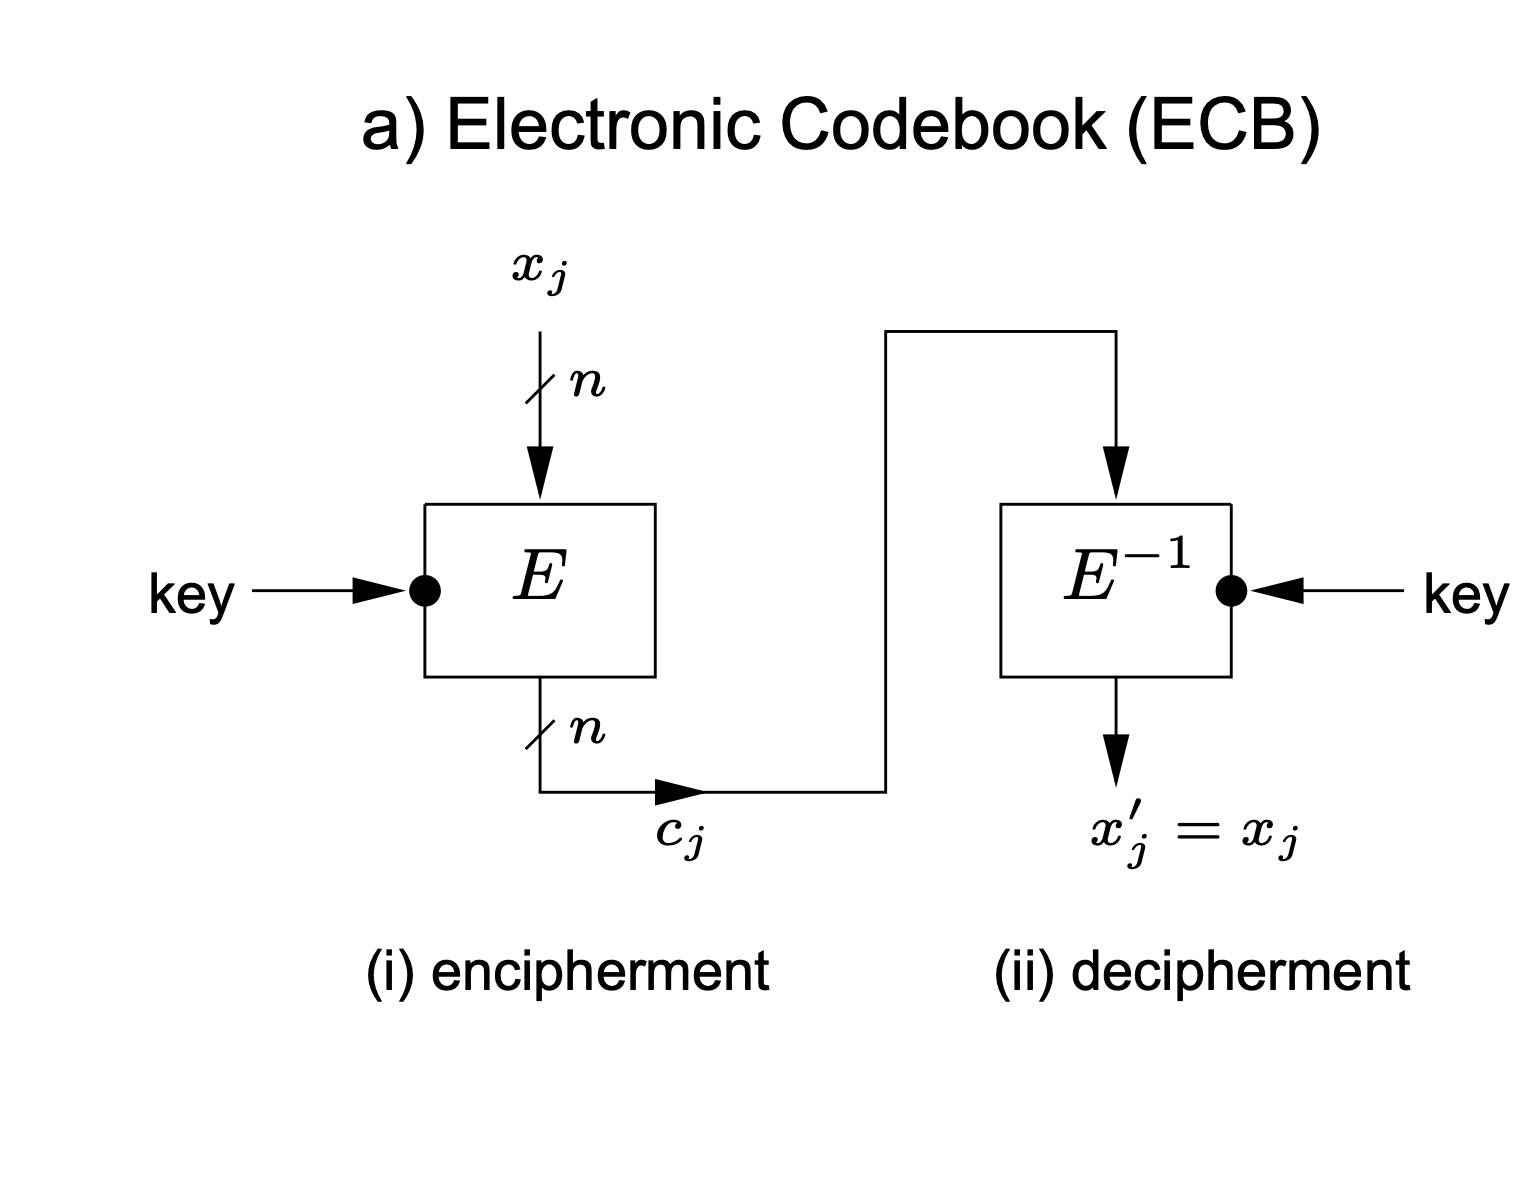
\includegraphics[width=0.45\textwidth]{ECB}
          \caption{\cite{Meneces}}
        \end{figure}

        \vfill

        \subsubsection{Cipher Block Chaining (CBC)}
      
        Cipher block chaining or CBC is an advancement made on ECB since 
        ECB compromises some security requirements. In CBC, previous cipher block is
        given as input to next encryption algorithm after XOR with original plaintext block. 
        In a nutshell here, a cipher block is produced by encrypting a XOR output of previous
        cipher block and present plaintext block. 

        \begin{figure}[!htbp] 
          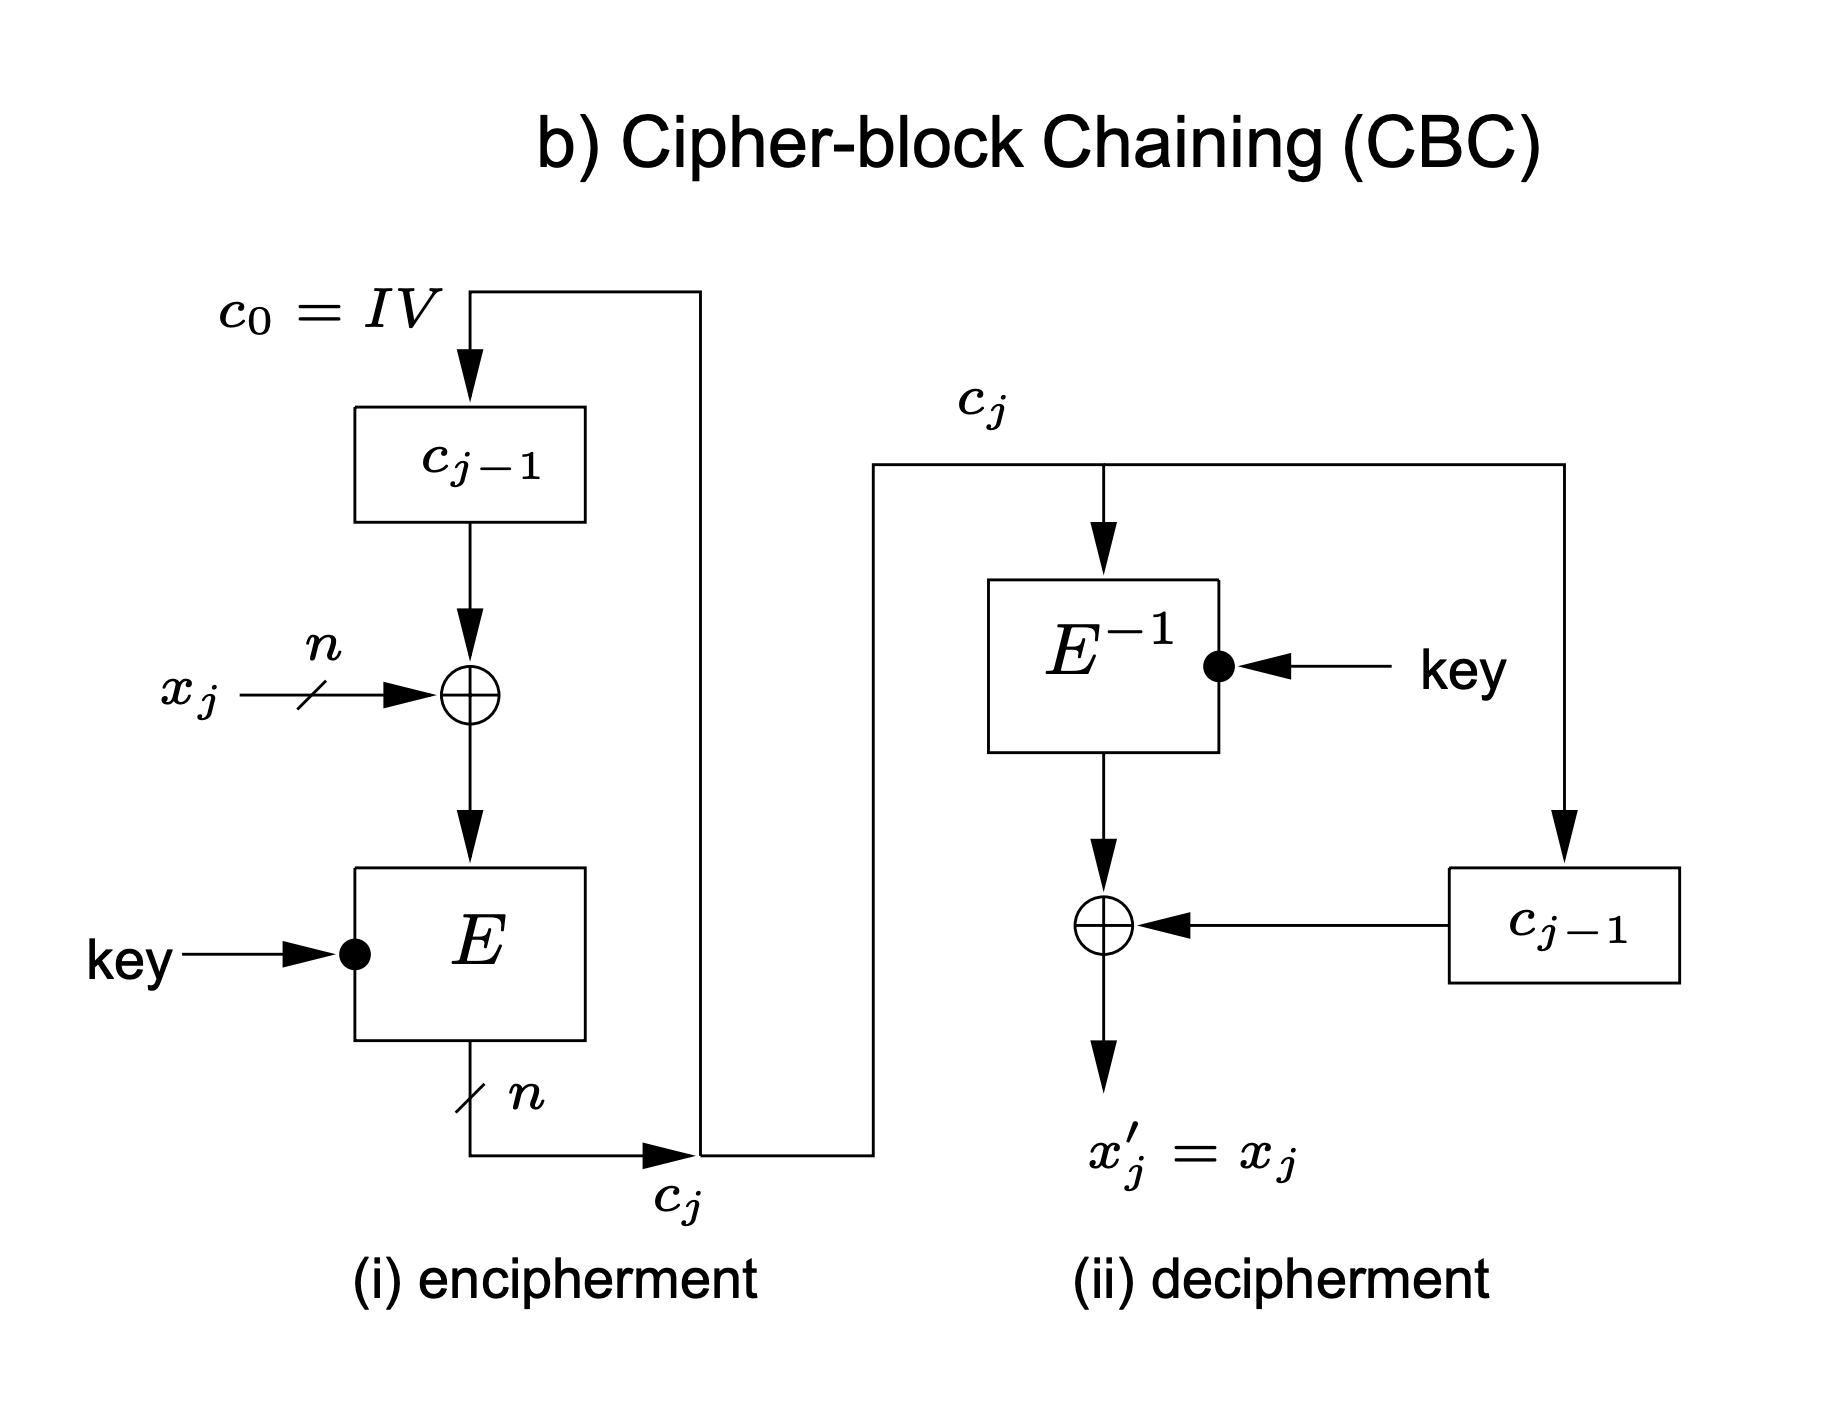
\includegraphics[width=0.45\textwidth]{CBC}
          \caption{\cite{Meneces}}
        \end{figure}

      \subsubsection{Cipher Feedback Mode (CFB)}
      
        In this mode the cipher is given as feedback to the next block of encryption with some new specifications: 
        first an initial vector IV is used for first encryption and output bits are divided as set of sandb-s bits
        the left hand side sbits are selected and are applied an XOR operation with plaintext bits. The result given
        as input to a shift register and the process continues. The encryption and decryption process for the same
        is shown below, both of them use encryption algorithm.

        \begin{figure}[!htbp] 
          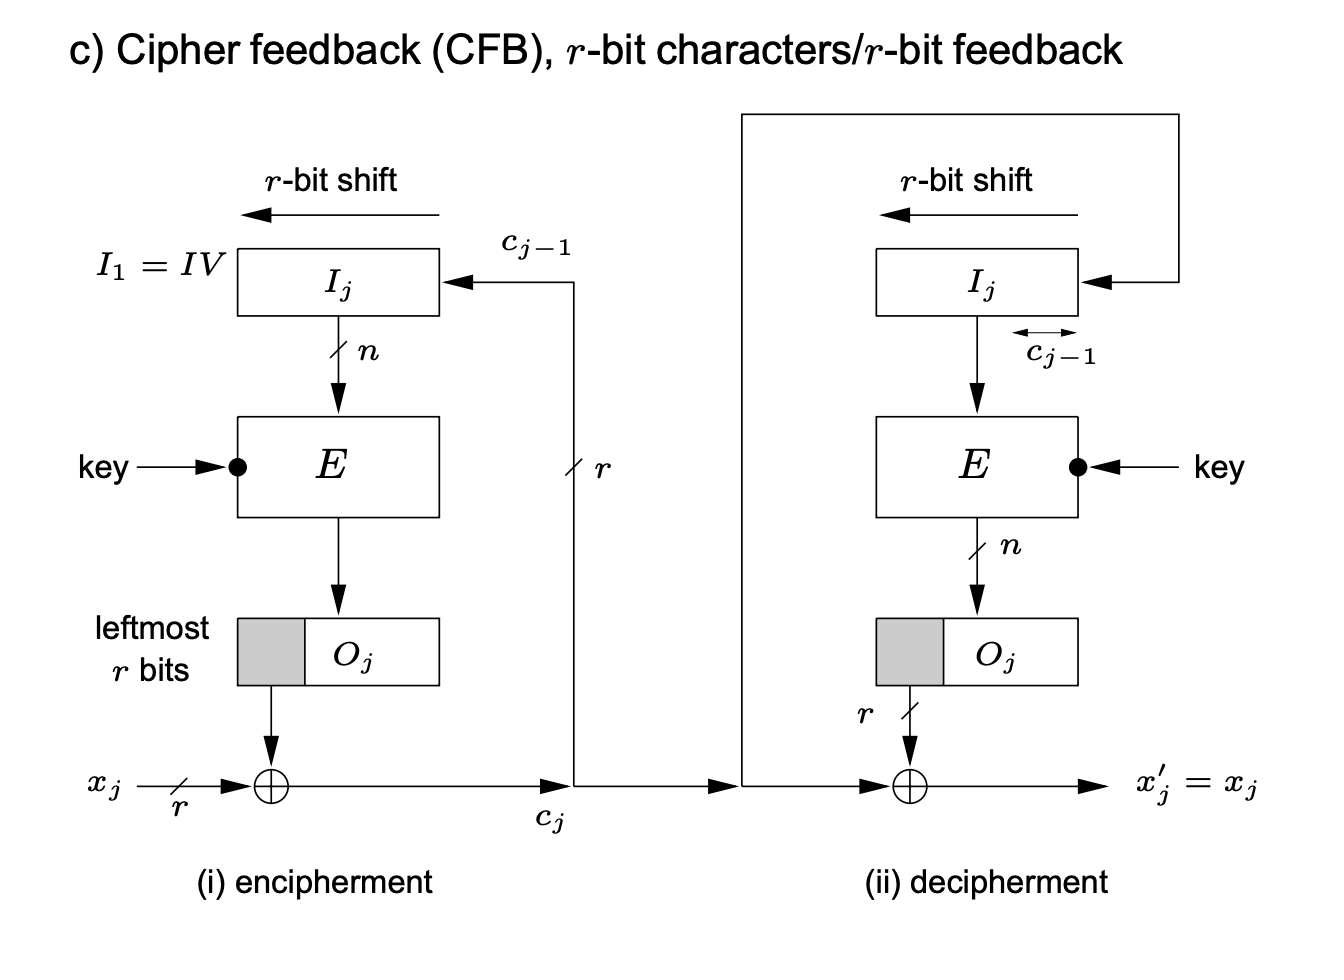
\includegraphics[width=0.45\textwidth]{CFB}
          \caption{\cite{Meneces}}
        \end{figure}


      Output Feedback Mode (OFB) 
      
        The output feedback mode follows nearly same process as the Cipher Feedback mode except that it sends
        the encrypted output as feedback instead of the actual cipher which is XOR output. In this output feedback
        mode, all bits of the block are send instead of sending selected s bits. The Output Feedback mode of block
        cipher holds great resistance towards bit transmission errors. It also decreases dependency or relationship
        of cipher on plaintext.

        \begin{figure}[!htbp] 
          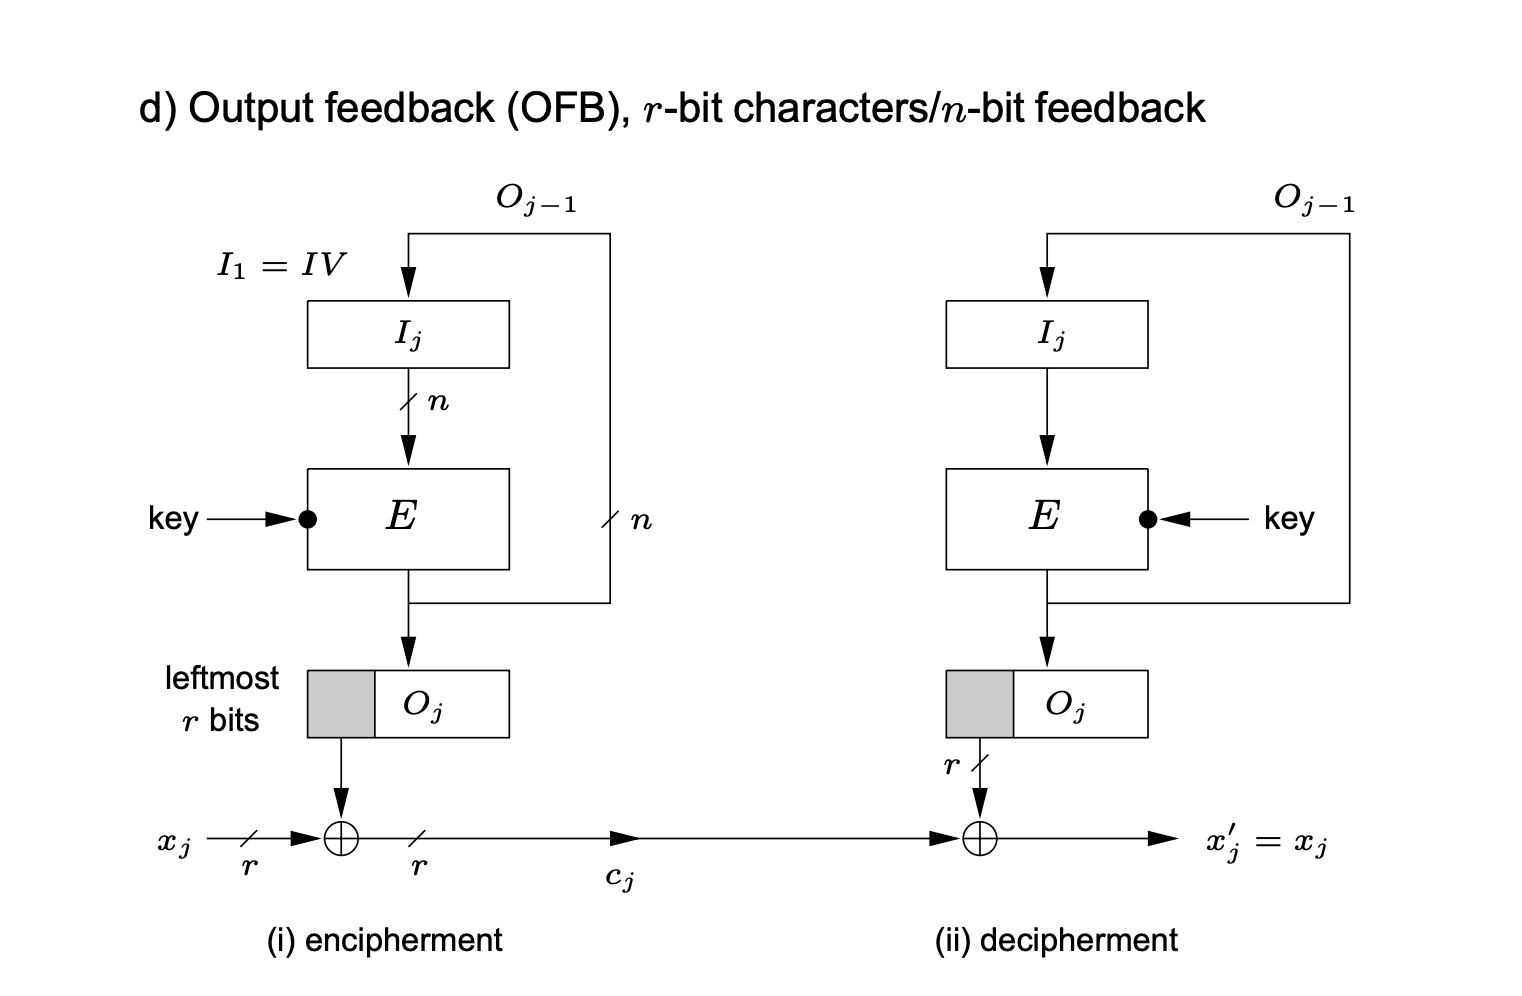
\includegraphics[width=0.45\textwidth]{OFB}
          \caption{\cite{Meneces}}
        \end{figure}


    \cite{GOG}

    \subsection{Initialization vector (IV)}

      An initialization vector (IV) or starting variable is a block of bits that is used by several modes to
      randomize the encryption and hence to produce distinct ciphertexts even if the same plaintext is
      encrypted multiple times, without the need for a slower re-keying process.

      An initialization vector has different security requirements than a key, so the IV usually does not
      need to be secret. However, in most cases, it is important that an initialization vector is never
      reused under the same key. For CBC and CFB, reusing an IV leaks some information about the first
      block of plaintext, and about any common prefix shared by the two messages. For OFB and CTR, reusing
      an IV completely destroys security.

      \cite{Wiki}


    \subsection{Padding}

      A block cipher works on units of a fixed size (known as a block size), but messages come in a variety of lengths.
      So some modes (namely ECB and CBC) require that the final block be padded before encryption. Several padding schemes exist.
      The simplest is to add null bytes to the plaintext to bring its length up to a multiple of the block size,
      but care must be taken that the original length of the plaintext can be recovered.

      \cite{Wiki}

  

  \section{Sotware}

    \begin{itemize}
      \item Python FLask  \cite{Flask}
      \item React JS  \cite{React}
      \item Python Pycryptodome \cite{Pycryptodome}
    \end{itemize}

  \section{Procedure}

    \begin{itemize}
      \item Create a simple SPA with react that is able to send a form with a file (bmp image) to a server (in this case localhost::5000/), 
      using POST, also add the algorithm and the operation mode desired.

      \item Create a simple server using Flask, with just one route, the root, in the case we get a request from GET, return the react app
      in case there is a POST request check to see if there is a file.

      \item If there is, upload the file to the server and save the filename
      \item Create a new copy of the saved image
      \item Use PIL to extract the pixel data and transform that to a array of bytes.
      \item Use Pycryptodome to create a helper function that accepts the array, uses padding and the IV if necessary.
      \item Recover the algorithm and the operation mode from the client and call the apropiate function.
      \item Store the new image in the server, return a link to that image to the client.
      \item Client need to show that image.
      
    \end{itemize}
  

  \section{Results and evidence}

    \begin{figure}[h]
      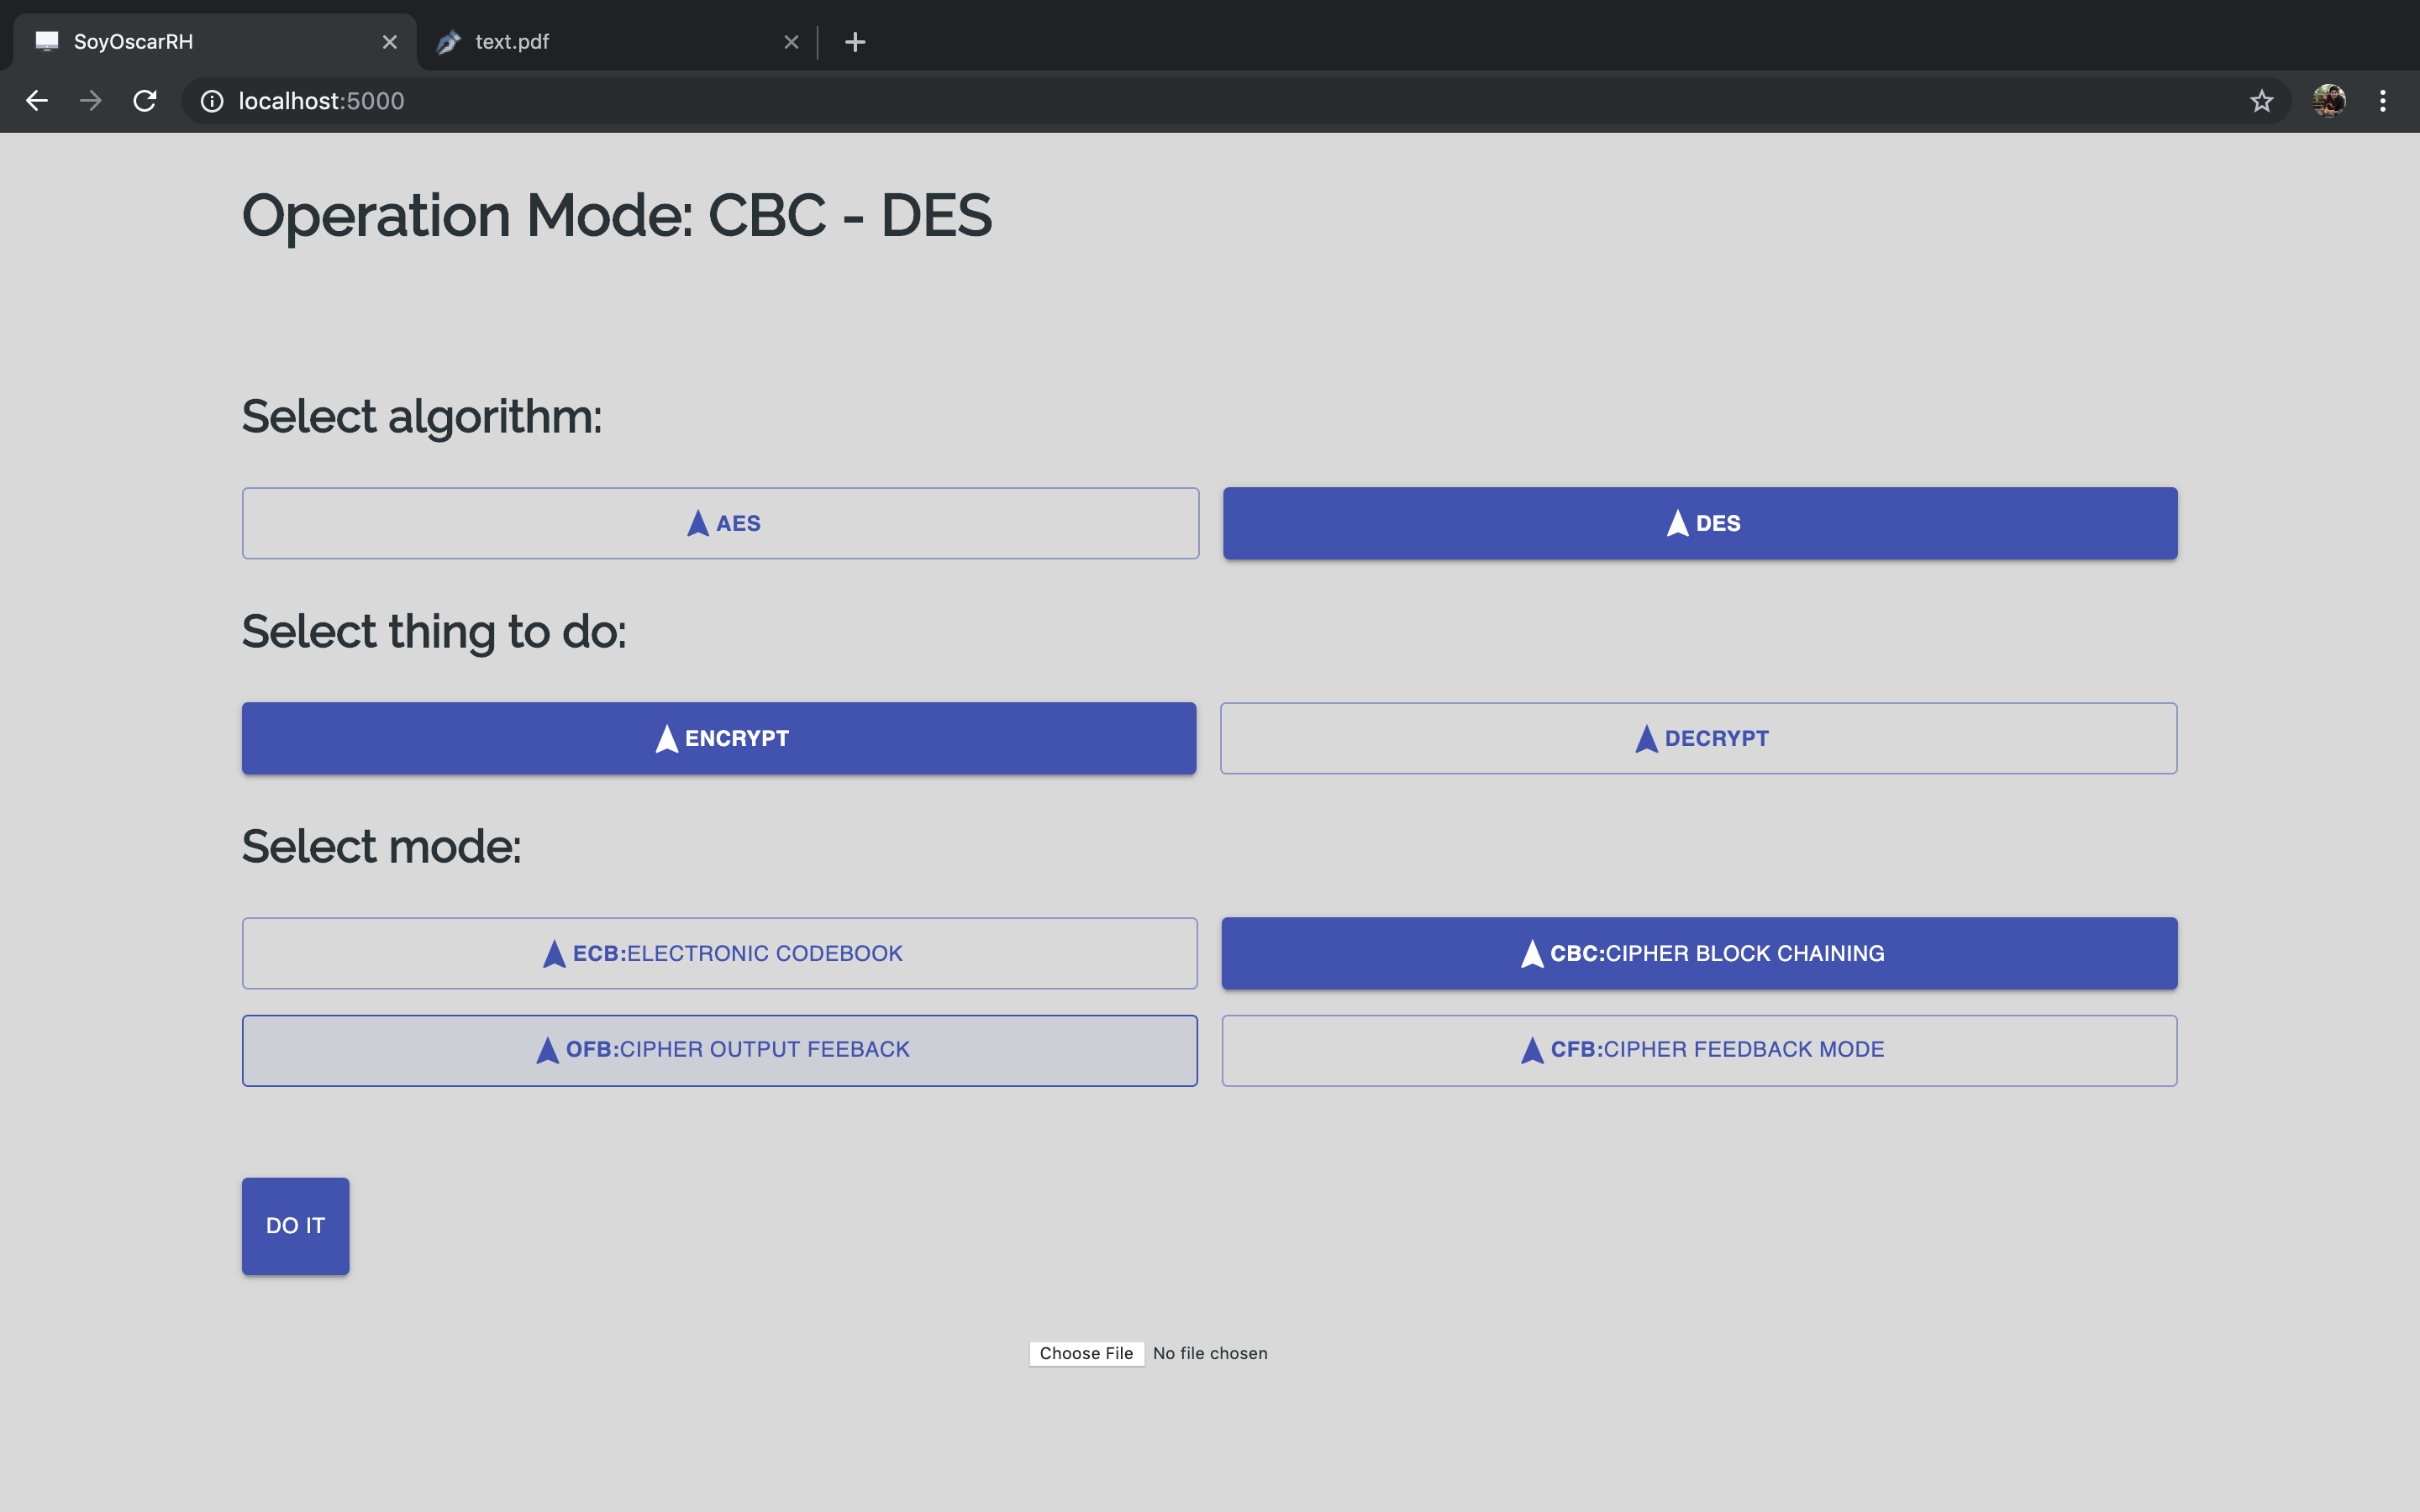
\includegraphics[width=0.65\textwidth]{data1}
      \caption{Screeenshots}
    \end{figure}

    \begin{figure}[h]
      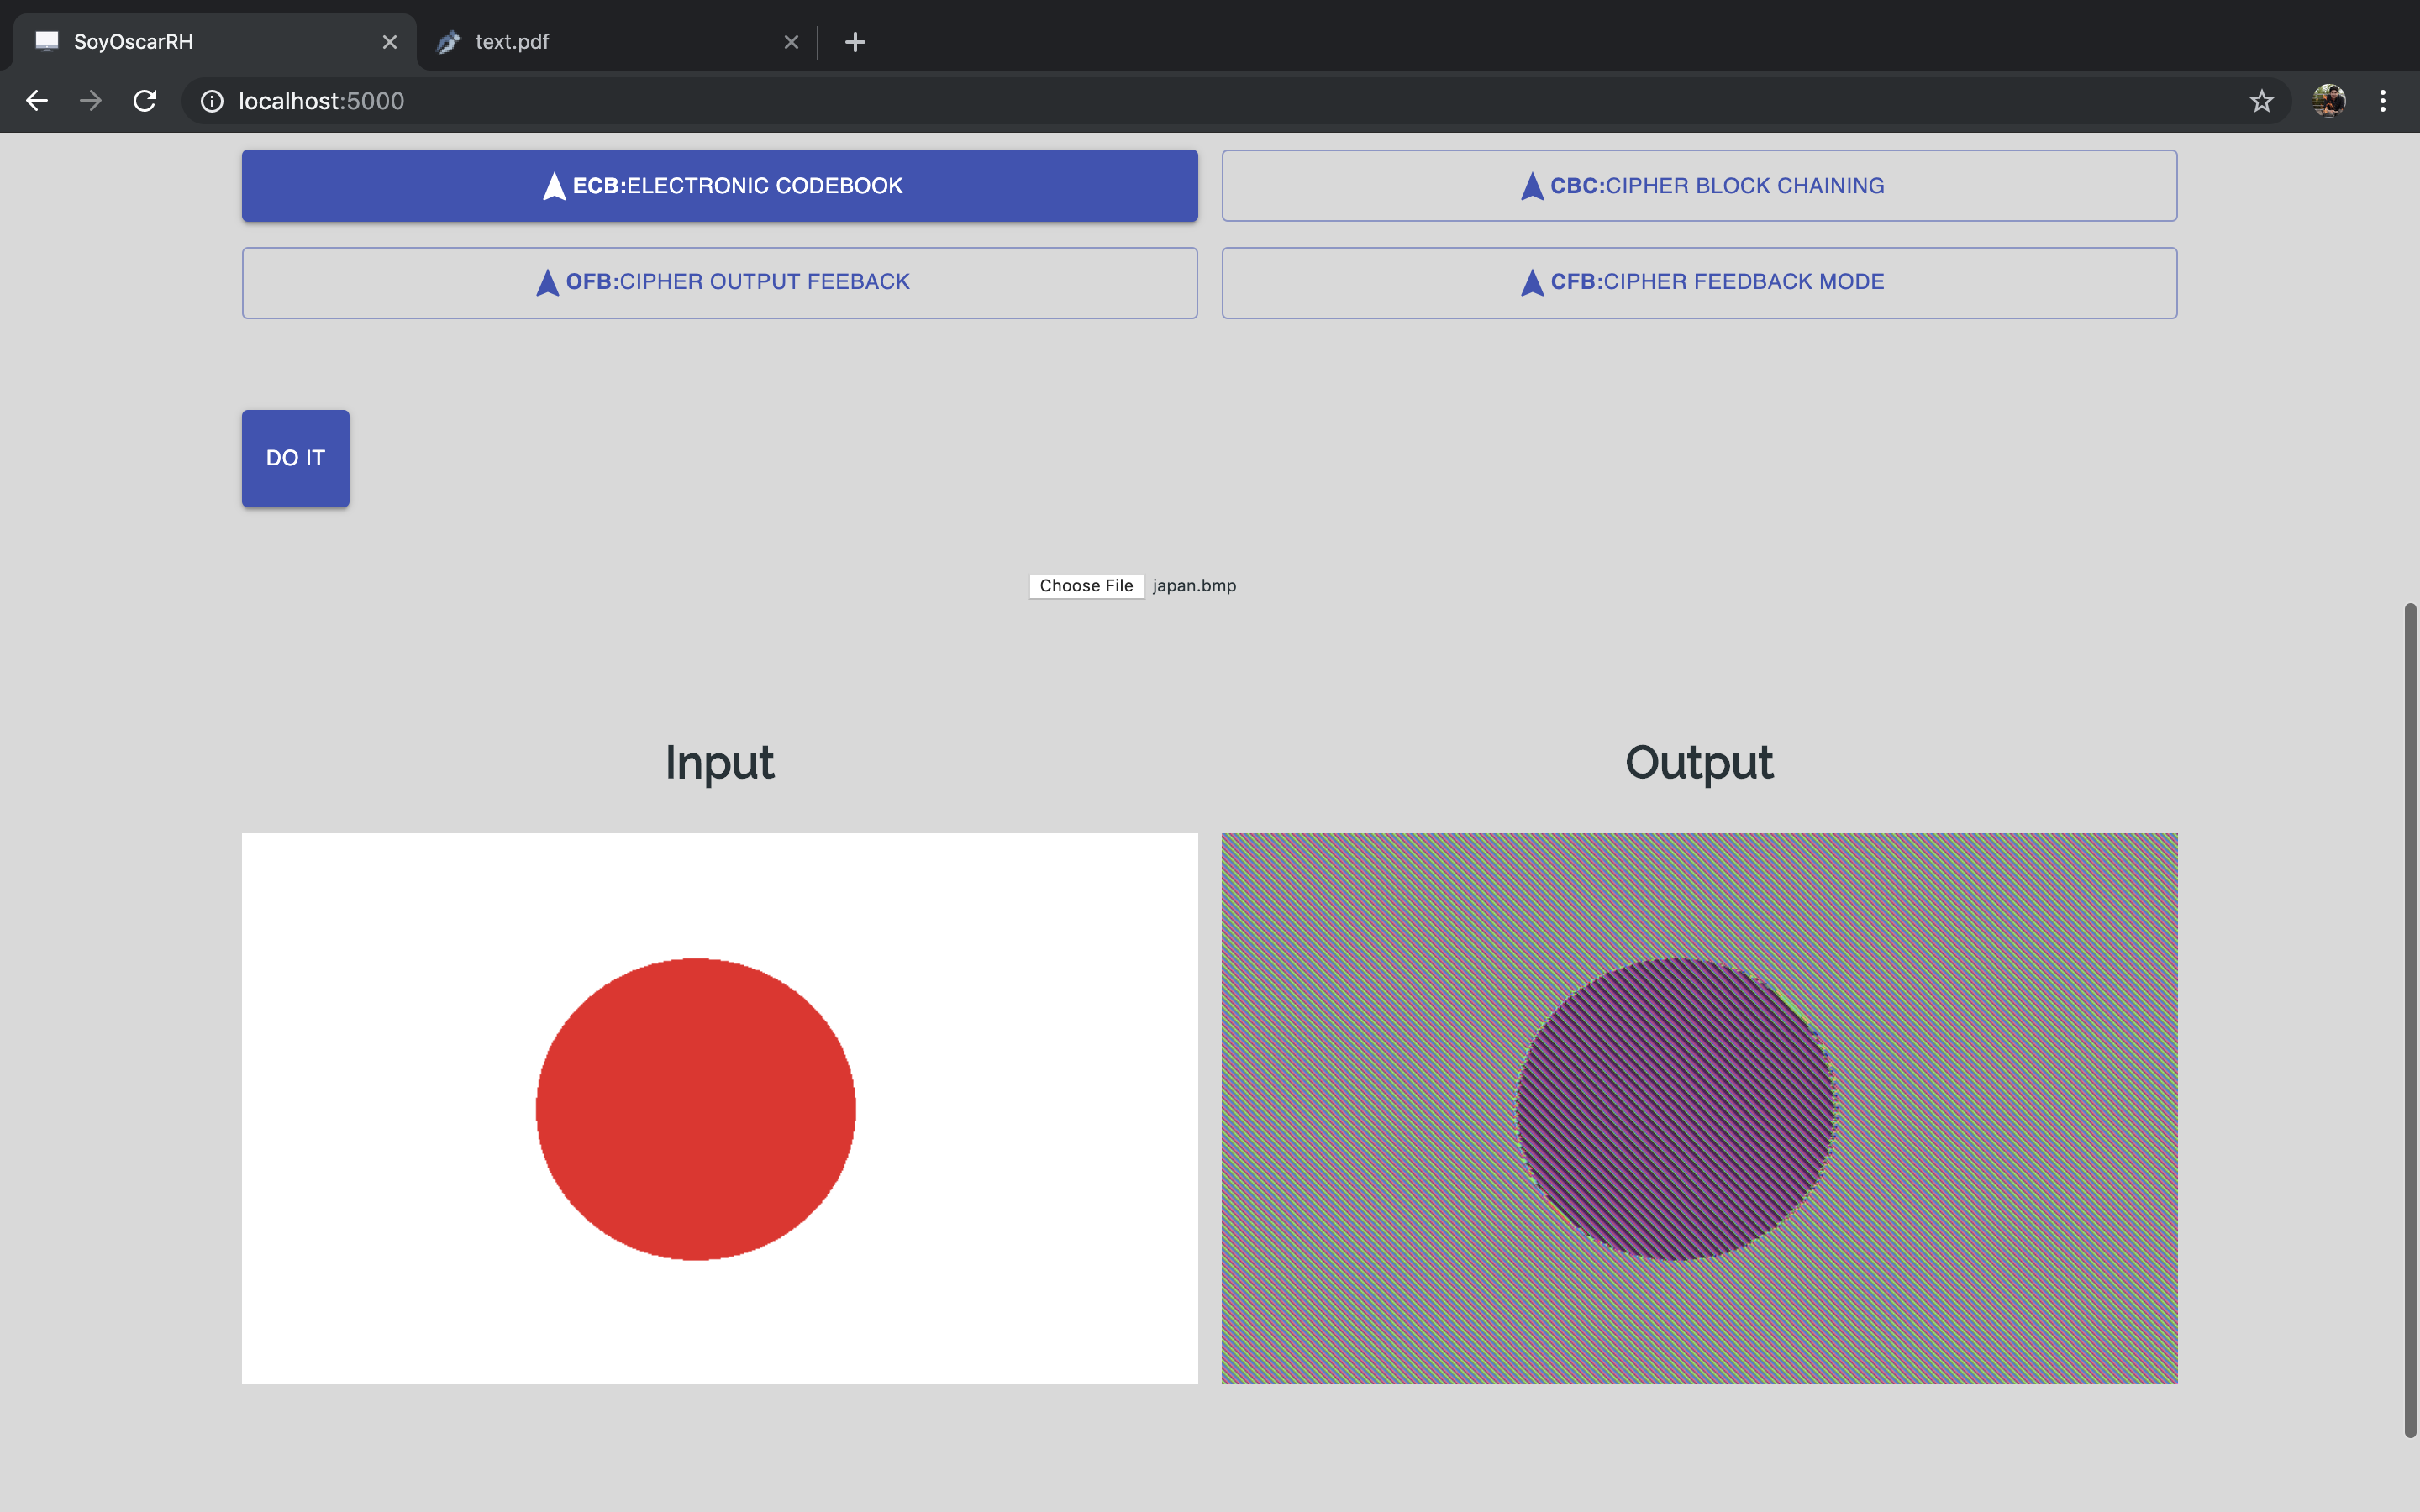
\includegraphics[width=0.65\textwidth]{data2}
      \caption{Screeenshots}
    \end{figure}

    \begin{figure}[h]
      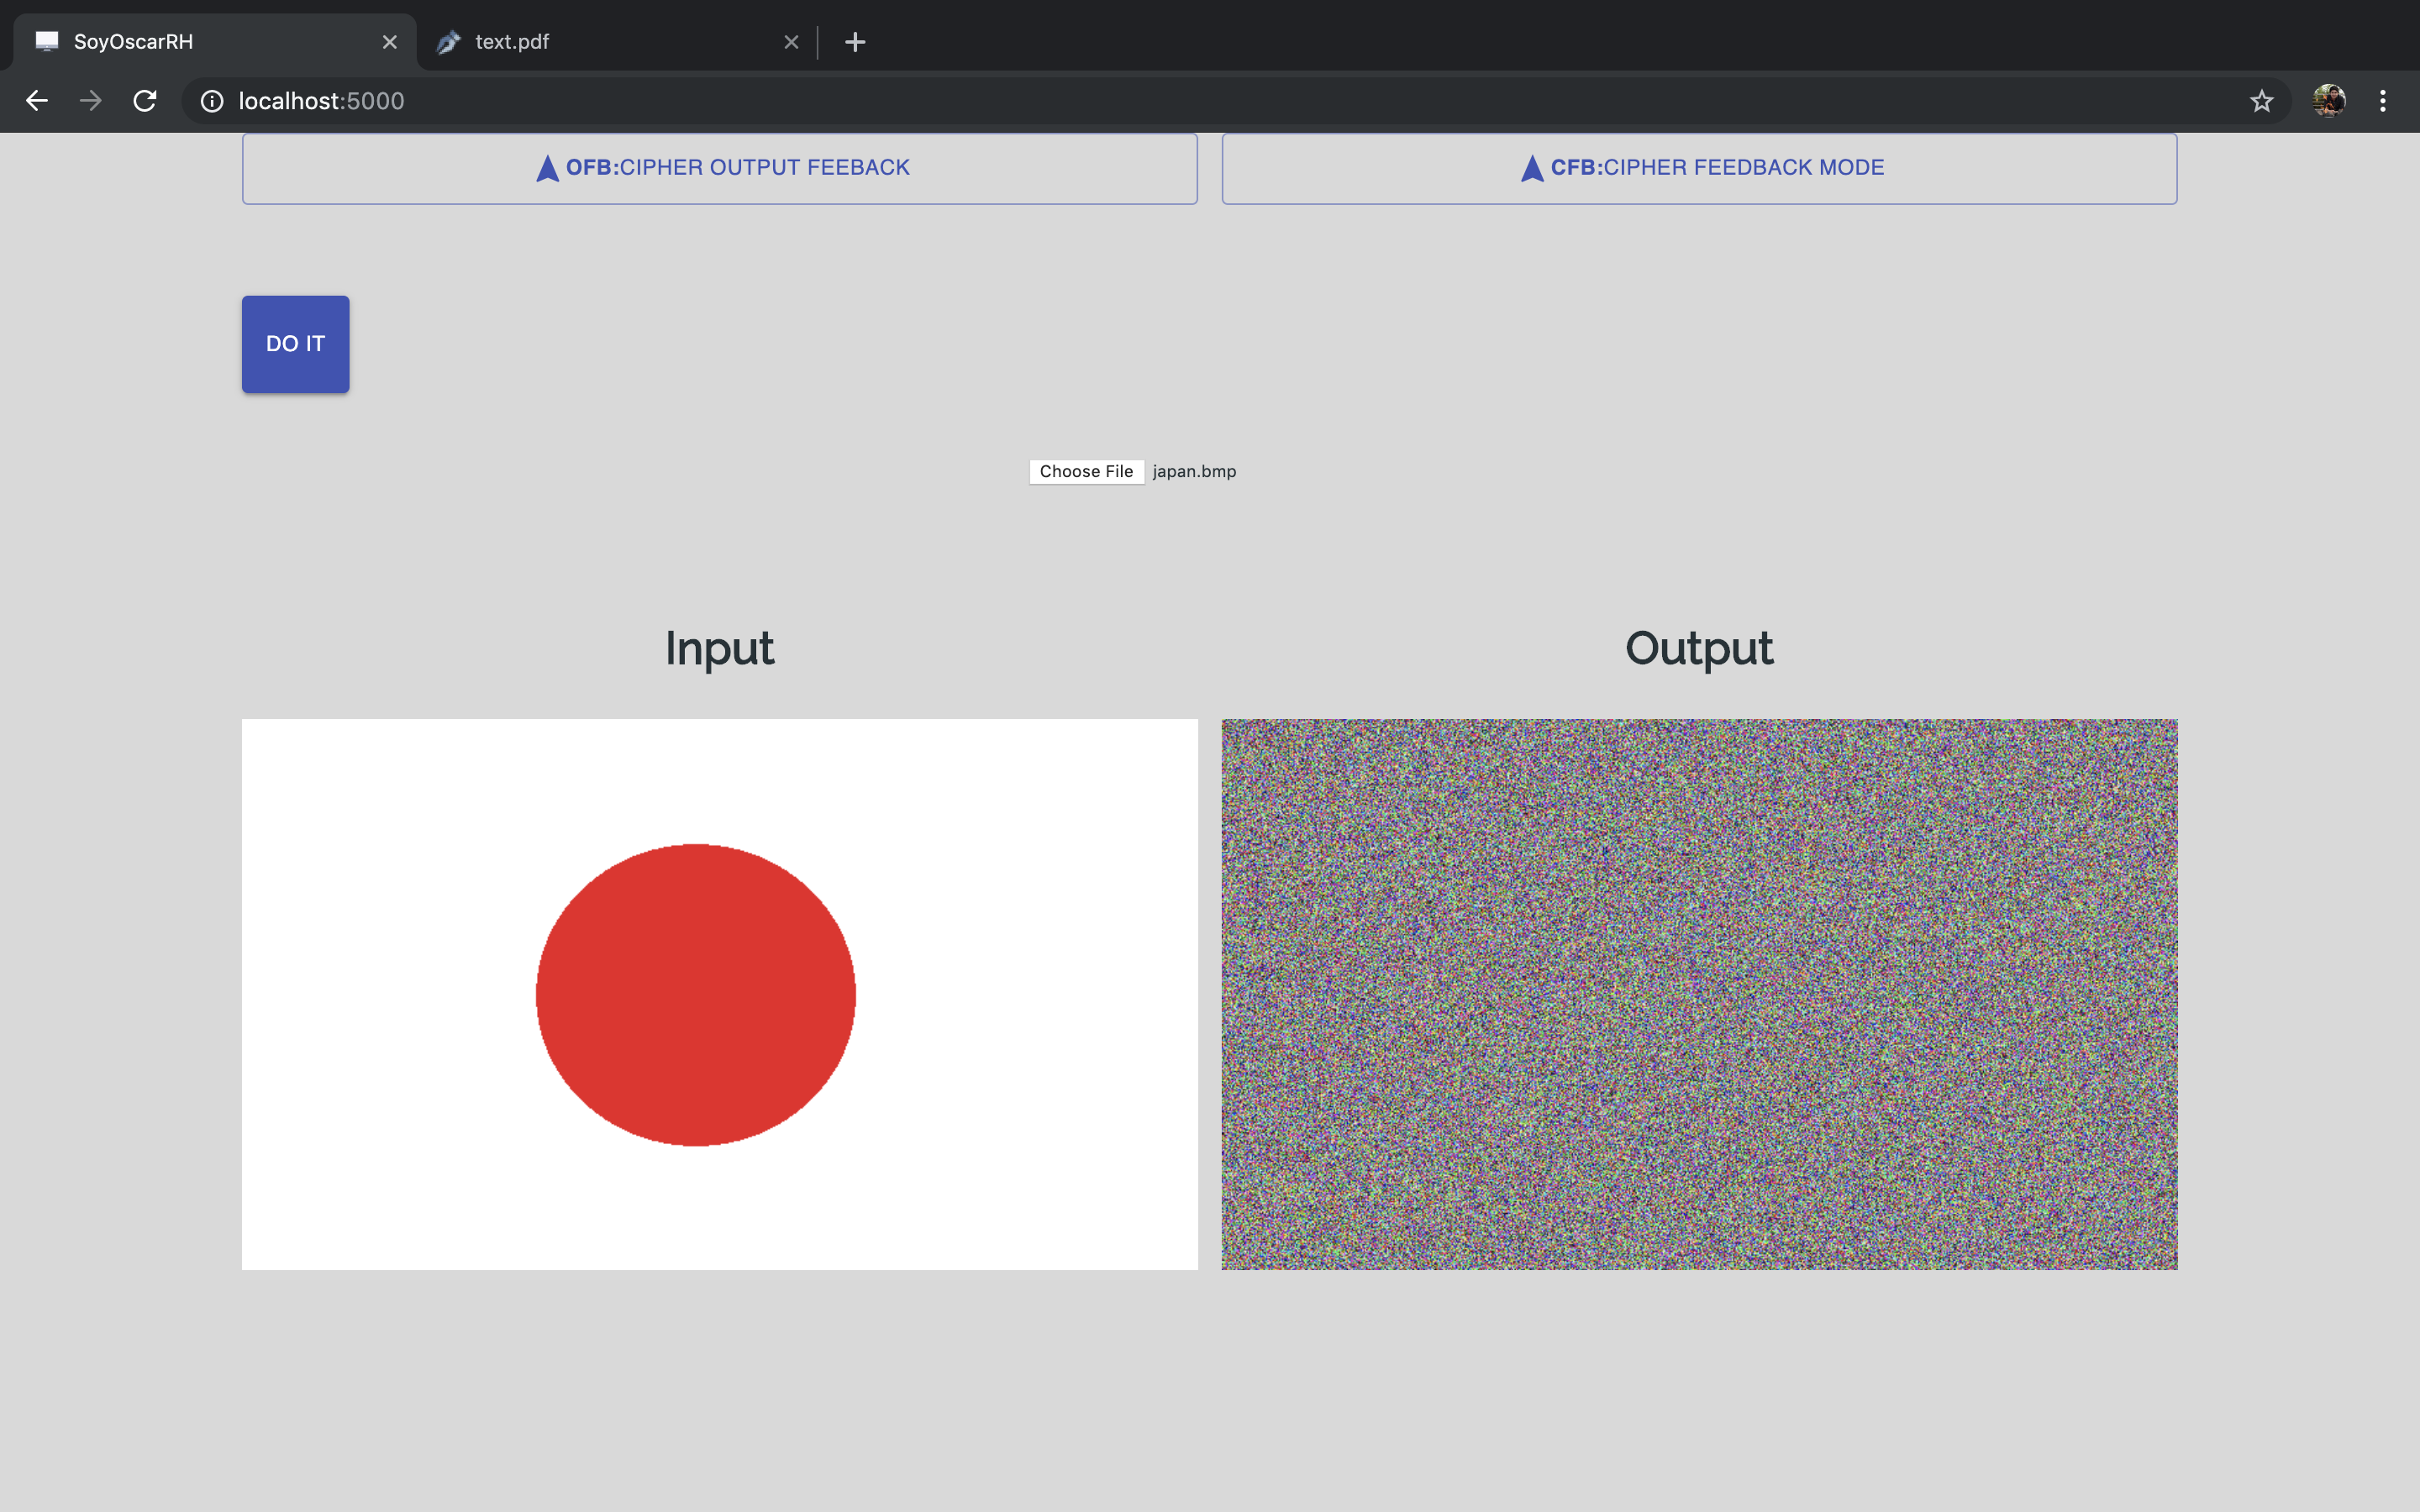
\includegraphics[width=0.65\textwidth]{data3}
      \caption{Screeenshots}
    \end{figure}


    \begin{tabular}{|r || p{5cm} | p{5cm} | }
      % And this is the name of all the headers
      \hline
      Mode & Image A & Image B  \\ [0.5ex] 
      \hline\hline
     
      %Body
        Original  &  
        \begin{minipage}{.2\textwidth}
          
\includegraphics[width=\linewidth]{japan}
        \end{minipage}  & 
        \begin{minipage}{.2\textwidth}
          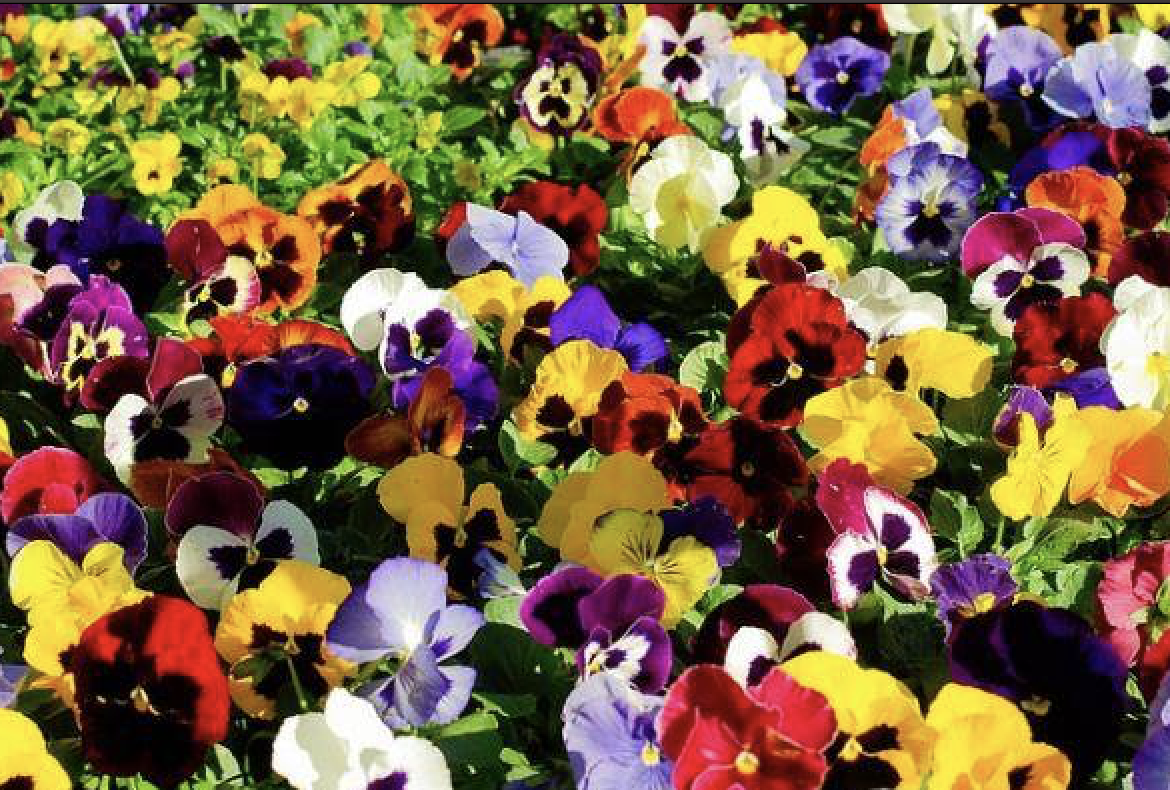
\includegraphics[width=\linewidth]{flores}
        \end{minipage}    
        \\\hline
        AES - ECB  &  
        \begin{minipage}{.2\textwidth}
          
\includegraphics[width=\linewidth]{1AES1}
        \end{minipage}  & 
        \begin{minipage}{.2\textwidth}
          
\includegraphics[width=\linewidth]{2AES1}
        \end{minipage}    
        \\\hline
        AES - CBC  &  
        \begin{minipage}{.2\textwidth}
          
\includegraphics[width=\linewidth]{1AES2}
        \end{minipage}  & 
        \begin{minipage}{.2\textwidth}
          
\includegraphics[width=\linewidth]{2AES2}
        \end{minipage}    
        \\\hline
        AES - CFB  &  
        \begin{minipage}{.2\textwidth}
          
\includegraphics[width=\linewidth]{1AES3}
        \end{minipage}  & 
        \begin{minipage}{.2\textwidth}
          
\includegraphics[width=\linewidth]{2AES3}
        \end{minipage}    
        \\\hline
        AES - OFB  &  
        \begin{minipage}{.2\textwidth}
          
\includegraphics[width=\linewidth]{1AES4}
        \end{minipage}  & 
        \begin{minipage}{.2\textwidth}
          
\includegraphics[width=\linewidth]{2AES4}
        \end{minipage}    
        \\\hline
   \end{tabular}


   \begin{tabular}{|r || p{5cm} | p{5cm} | }
    % And this is the name of all the headers
    \hline
    Mode & Image A & Image B  \\ [0.5ex] 
    \hline\hline
   
    %Body
      Original  &  
        \begin{minipage}{.2\textwidth}
          
\includegraphics[width=\linewidth]{japan}
        \end{minipage}  & 
        \begin{minipage}{.2\textwidth}
          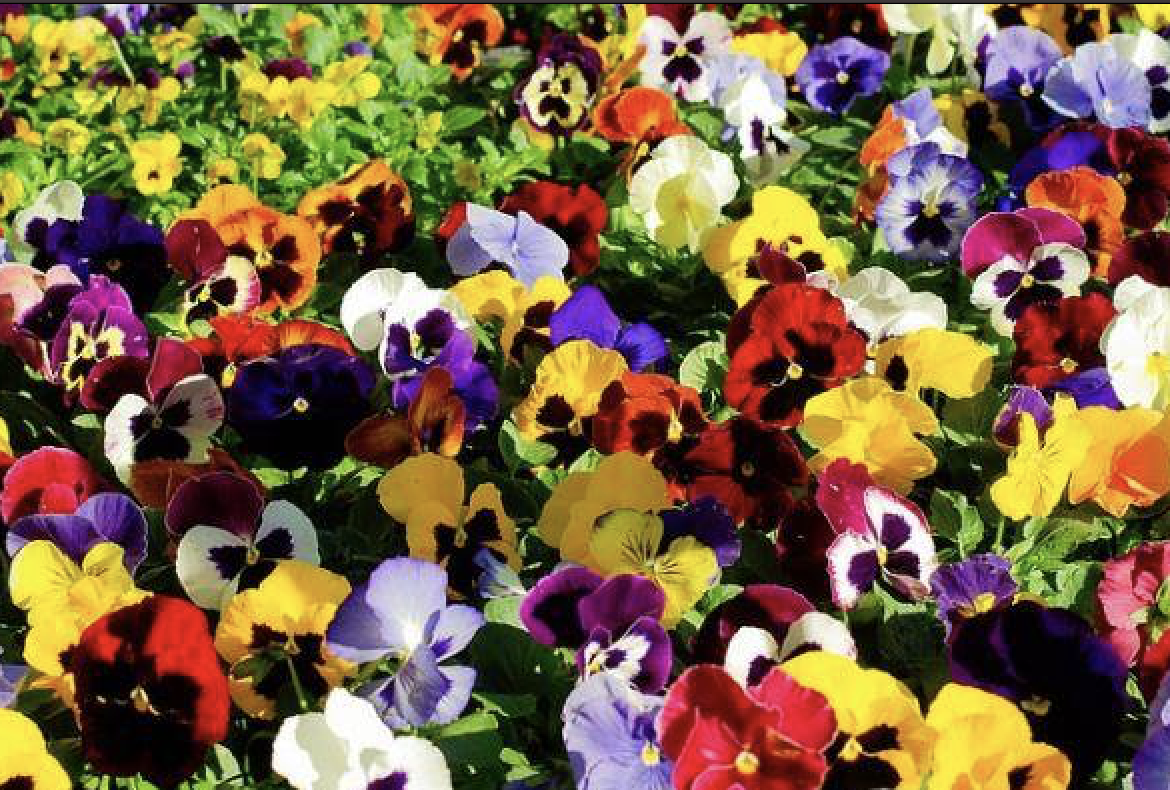
\includegraphics[width=\linewidth]{flores}
        \end{minipage}
        \\\hline
      DES - ECB  &  
      \begin{minipage}{.2\textwidth}
        
\includegraphics[width=\linewidth]{1DES1}
      \end{minipage}  & 
      \begin{minipage}{.2\textwidth}
        
\includegraphics[width=\linewidth]{2DES1}
      \end{minipage}    
      \\\hline
      DES - CBC  &  
      \begin{minipage}{.2\textwidth}
        
\includegraphics[width=\linewidth]{1DES2}
      \end{minipage}  & 
      \begin{minipage}{.2\textwidth}
        
\includegraphics[width=\linewidth]{2DES2}
      \end{minipage}    
      \\\hline
      DES - CFB  &  
      \begin{minipage}{.2\textwidth}
        
\includegraphics[width=\linewidth]{1DES3}
      \end{minipage}  & 
      \begin{minipage}{.2\textwidth}
        
\includegraphics[width=\linewidth]{2DES3}
      \end{minipage}    
      \\\hline
      DES - OFB  &  
      \begin{minipage}{.2\textwidth}
        
\includegraphics[width=\linewidth]{1DES4}
      \end{minipage}  & 
      \begin{minipage}{.2\textwidth}
        
\includegraphics[width=\linewidth]{2DES4}
      \end{minipage}    
      \\\hline
 \end{tabular}


  \section{Discussion}

    We can see that with CBC parallel encryption of blocks of bits is possible, thus it is a faster way of encryption,
    but prone to cryptanalysis since there is a direct relationship between plaintext and ciphertext.

    CBC is better resistive nature towards cryptanalsis than ECB, in general, every operation mode is better that 
    ECB.

  \section{Conclusions}

    I learned a lot about operation mode, what does it mean to have padding why OFB does not need it, and the different size of
    key and IV in AES and DES (also, that explain a little bit with it is not recomended to use DES).

    The software that I developted will work with any of the former operation modes and any BMP image.

  \section{Code}

    See it in: https://github.com/SoyOscarRH/LibroCriptografia/tree/master/Code/OperationModes
    
    \lstinputlisting[gobble=4, language=JavaScript]{../Code/App/index.tsx}
    \lstinputlisting[gobble=4, language=python]{../app.py}




  \begin{thebibliography}{10}

      \bibitem{GOG} 
        Block Cipher modes of Operation
          \textit{https://www.geeksforgeeks.org/block-cipher-modes-of-operation/}. 

      \bibitem{Wiki} 
        Block cipher mode of operation - Wikipedia
          \textit{$https://en.wikipedia.org/wiki/Block_cipher_mode_of_operation/$}. 
  
      \bibitem{Meneces} 
        Handbook of Applied Cryptography, 
        Alfred J. Menezes,
        Paul C. van Oorschot,
        Scott A. Vanstone 

      \bibitem{Flask} 
        \textit{http://flask.palletsprojects.com/en/1.1.x/}. 

      \bibitem{React} 
        \textit{https://reactjs.org/}. 

      \bibitem{Pycryptodome} 
        \textit{https://pycryptodome.readthedocs.io/en/latest/index.html}. 



  \end{thebibliography}

\end{document}